\item \points{3d} \textbf{Coding problem: re-weighting minority class}

In \texttt{src-imbalanced/submission.py}, implement the logistic regression algorithm on $\calD'$.  Compute and report the classifier's accuracy ($A$), balanced accuracy ($\overline{A}$), accuracies for the two classes ($A_0, A_1$) on the validation dataset. You are expected to see that the accuracy of minority class (class 1) improved significantly whereas that of the majority class dropped compared to vanilla logistic regression. However, the balanced accuracy is significantly greater than that of the vanilla logistic regression. 

Please adjust the |apply_logistic_regression| you worked with in 3b to capture the reweighted minority class solution. 
Then fill in the |upsample_minority_class| function. 

The output plot should look similar to the following (no plot submission is required):

\begin{figure}[H]
	\centering
	\vspace{2mm}
	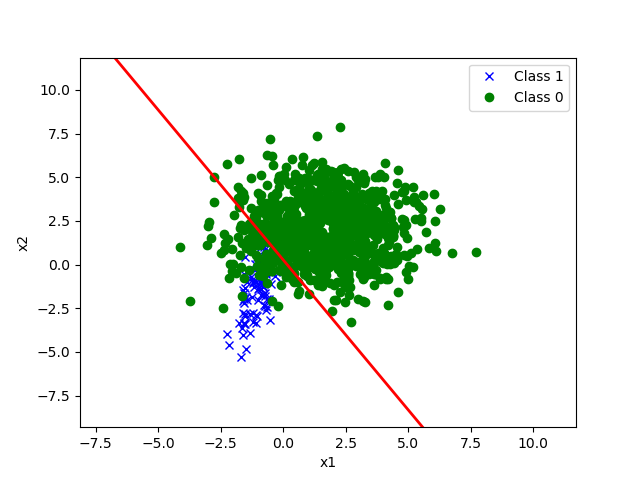
\includegraphics[width=0.5\linewidth]{03-imbalanced/imbalanced_upsampling_pred.png}
	  \caption{Validation set with $x_1$ on the horizontal axis and $x_2$ on
	  the vertical axis. The decision boundary obtained by your model (i.e, line corresponding to model's predicted probability = 0.5). Visual impaired students can access the corresponding desmos plot \href{https://www.desmos.com/calculator/yzewr1djk7}{here}}
  \end{figure}